\acused{KNN}
\label{chap:KNNs}
Durch künstliche neuronale Netze (\acsp{KNN}) können Maschinen lernen, bestimmte Probleme zu lösen, ohne dass ein Mensch vorher explizite Regeln dafür definieren muss. Dies steht im Kontrast zur Methode, der Maschine  vorher einen festen, vollständigen Regelsatz bereitzustellen. Letztgenannter Ansatz zeigt in einigen Gebieten nur begrenzten Erfolg, da es für Menschen herausfordernd sein kann, Regelsätze für Vorgänge zu definieren, die unbewusst im Gehirn stattfinden oder viel Kontext erfordern. Zu nennen sind hierbei die visuelle Objekterkennung oder menschliche Sprache. Außerdem können neue, nicht in den Regeln beachtete Situationen dazu führen, dass die Maschine das Problem nicht mehr lösen kann. Die Grundidee hinter \acp{KNN} ist deshalb, dass sich die Maschine selber einen Wissensschatz aufbaut, der ihr beim Lösen des Problems hilft. Dies geschieht, indem die Entwickler ihr reale Trainingsbeispiele zeigen. Möchte man einen Algorithmus trainieren, der Schach spielen soll, kann man ihm beispielsweise eine Vielzahl an realen Schachpartien zeigen. Anhand dessen lernt der Algorithmus verschiedene Strategien und baut ein Spielverständnis auf, das womöglich über die menschlichen Fähigkeiten hinausgeht. \cite[S. 1ff.]{DeepLearningBook}

In den letzten Jahrzehnten erlebte das maschinelle Lernen und damit auch das Gebiet der \acp{KNN} einen Aufschwung. Es existiert bereits seit Mitte des vergangenen Jarhunderts, wird allerdings erst durch die zunehmende Rechenleistung und die Verfügbarkeit von großen Datenmengen flächendeckend eingesetzt. Einsatzgebiete für \acp{KNN} sind unter anderem die Objekterkennung, das Verstehen von natürlicher Sprache und die Generierung von Text und Bildern. \cite[S. 4,17]{knnsKompakt}

Die Inspiration für \acp{KNN} bildet die Informationsverarbeitung des Gehirns in Lebewesen. Die kleinste hier betrachtete Einheit ist das Neuron. Neuronen in \acp{KNN} sind konzeptionell inspiriert von realen, biologischen Neuronen, besitzen aber eine deutlich abstrahierte Funktionsweise. In \acp{KNN} berechnen sie ein Skalarprodukt ihrer gewichteten Eingangswerte, addieren einen sogennaten \emph{Bias} hinzu und wenden auf das Ergebnis eine nichtlineare Funktion an. Letzere wird auch als Aktivierungsfunktion bezeichnet. Diese Aktivierungsfunktion kann analog dazu gesehen werden, dass biologische Neuronen einen Schwellenwert (\emph{engl.: threshold}) besitzen, der überschritten werden muss, damit das Neuron \emph{feuert}, also einen Impuls an weitere Neuronen weitergibt. Aktivierungsfunktionen sind notwendig, damit neuronale Netze Probleme lösen können, die über die Fähigkeiten einer linearen Regression hinausgehen. Es wird eine nichtlineare Abhängigkeit zwischen dem Eingang $X$ und dem Ausgang $Y$ umgesetzt. \cite{visualApproach}

In der Nachfolgenden Abbildung ist ein einzelnes künstliches Neuron eines \acp{KNN} darstellt. Das \emph{Plus-Zeichen} steht für die Berechnung des Skalarprodukts der Eingänge und der darauf addierte Bias. Die Aktivierungsfunktion wird durch das \emph{Sigmoid}-Zeichen simbolisiert. Der Ausgang (\emph{rechts}) ist das Ergebnis der Berechnung des Neurons. \cite{visualApproach}

\begin{figure}[H]
   \centering
   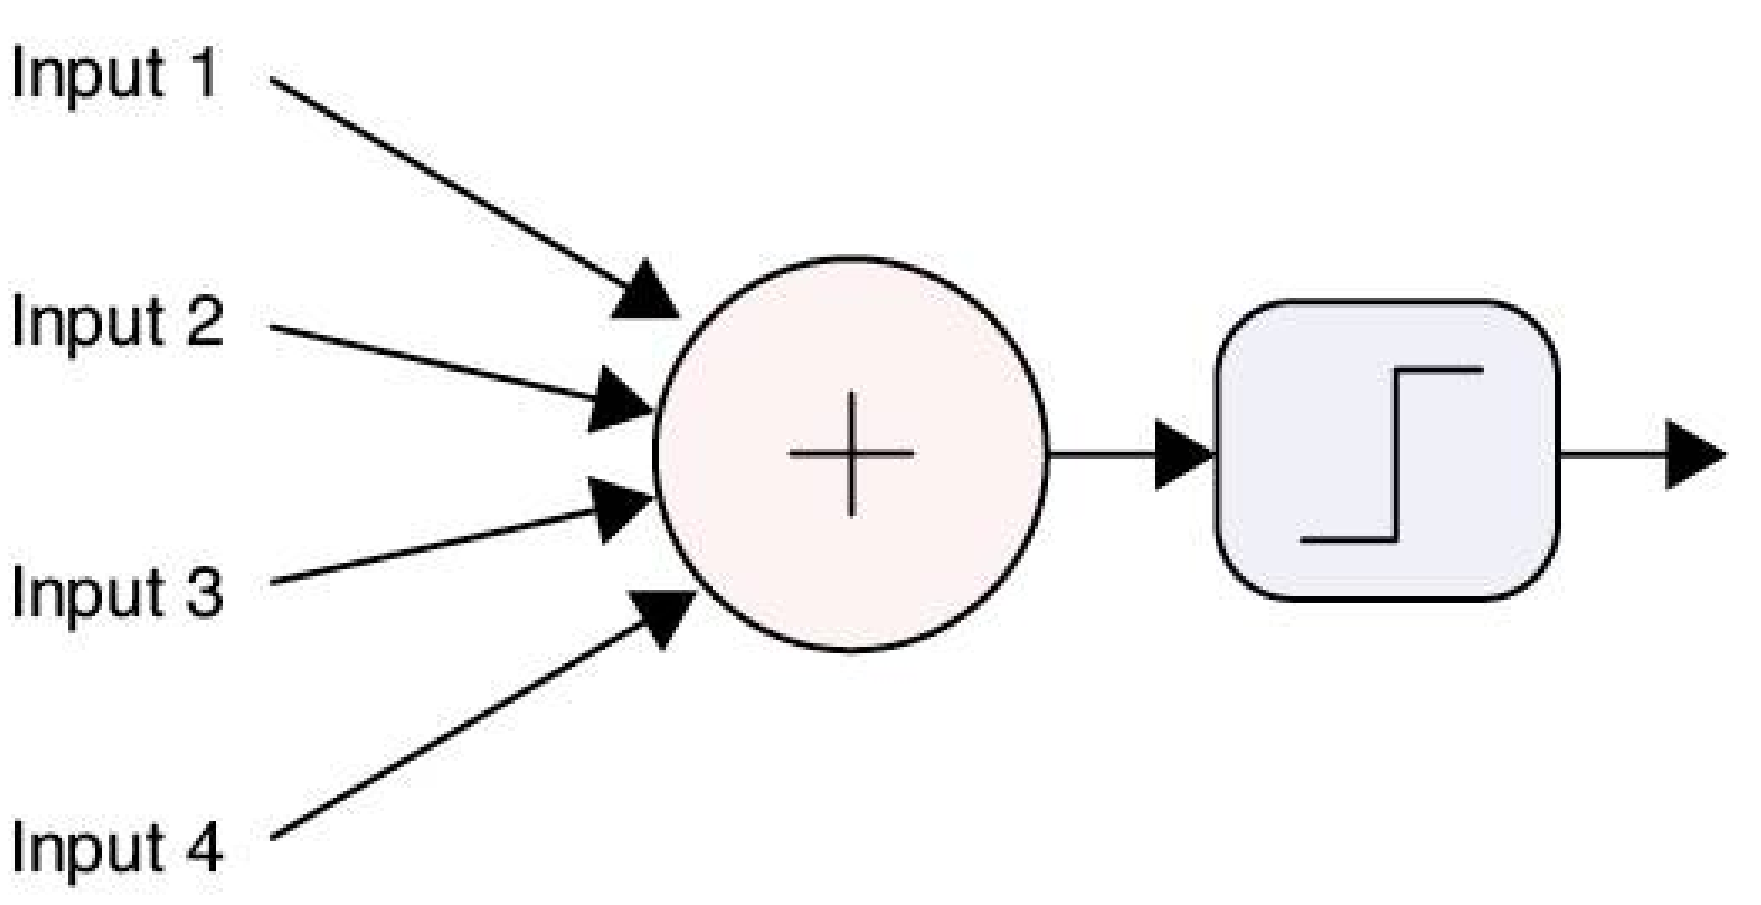
\includegraphics[width=0.5\textwidth]{images/KNNs/Neuron.png}
   \caption{Einzelnes Neuron eines \acp{KNN} \cite{visualApproach}}
\end{figure}

Um komplexe Probleme lösen zu können, werden mehre Neuronen miteinander verbunden und in Schichten angeordnet. Jede Schicht erhält die Ausgangswerte der vorherigen Schicht als Eingang und gibt die daraus berechneten, neuen Werte an die nächste Schicht weiter. In der nachfolgenden Abbildung sind die Neuronen durch Kreise dargestellt und ihre Verbindungen durch Linien. Eine Verbindung stellt dar, dass ein Neuron seinen berechneten Wert an das nachfolgende Neuron weitergibt. Dies geschieht hierbei ausschließlich von \emph{links nach rechts}, womit das \ac{KNN} als \emph{Feedforward-Netzwerk} bezeichnet wird. Die Eingabeschicht erhält die Eingabewerte des Netzwerks, die Ausgabeschicht liefert die Vorhersage des Modells. Zwischen diesen beiden Schichten befinden sich beliebig viele verarbeitende Schichten, die als \emph{Hidden Layer} bezeichnet werden. \cite{knnsKompakt}

\begin{figure}[H]
   \centering
   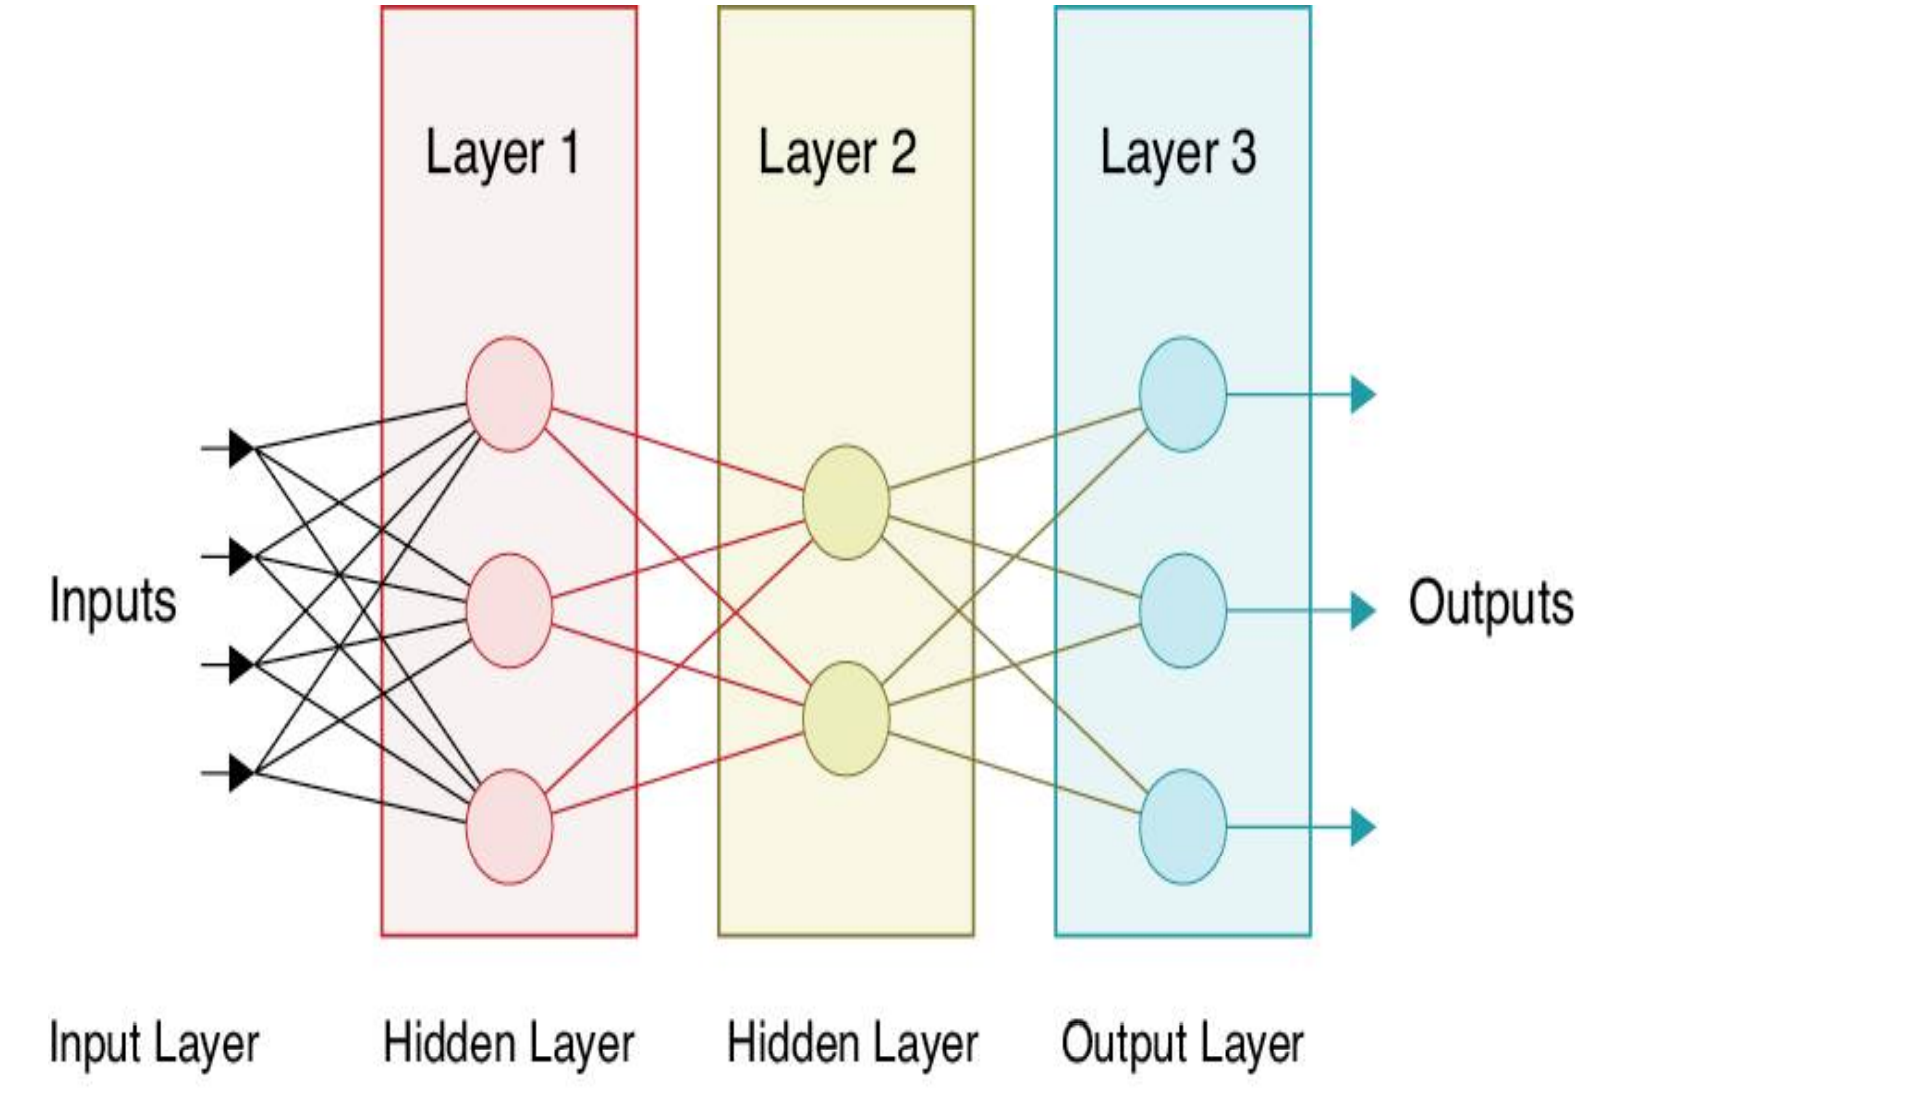
\includegraphics[width=0.7\textwidth]{images/KNNs/KNN_layers.png}
   \caption{Vollständiges \ac{KNN} \cite{visualApproach}}
\end{figure}

Die Vorhersage, gekennzeichnet durch die Werte der Ausgabeschicht, hängt von den jeweiligen Parametern der Neuronen des Netzwerks ab. Dies sind die Gewichte (\emph{engl.: weights}) der Verbindungen zwischen den Neuronen sowie der Bias der Neuronen. Es existieren auch trainierbare Aktivierungsfunktionen, diese sind jedoch vergleichsweise unüblich. Entwickler sind für den Entwurf der Netzwerkarchitektur zuständig, die Parameter werden jedoch durch das Modell trainiert. Zu Beginn besitzt das Modell zufällige Parameter, wodurch es in der Regel nicht die gewünschte Abbildung zwischen Ein- und Ausgabe implementiert. Ein untrainierter Schachalgorithmus spielt demnach augenscheinlich willkürliche Züge. Ein untrainierter Katzenklassifikator besitzt keinen erkennbaren Wissensschatz darüber, welche Charakteristiken eine Katze optisch auszeichnen. Das Ziel des Trainings ist, dass die Parameter des Modells zunehmend gegen das Optimum konvergieren und so das Modell immer plausibler in seinen Vorhersagen wird.

%---------------------------------------------------------------------------------------------------------------
\subsection{Training}
Damit ein neuronales Netz trainiert werden kann, bedarf es einer Funktion, die die Qualität der Vorhersagen des Modells bestimmt. Erst dadurch kann verglichen werden, ob eine gegebene Änderung der Parameter eine Annäherung an das globale Optimum zurfolge hat. Diese Funktion wird als \emph{Kostenfunktion} bezeichnet. Sie berechnet, gemittelt über alle $m$ Trainingsbeispiele $i$, die Abweichung des vorhergesagten Wertes $\hat{y}$ von dem tatsächlichen Wert $y$.
Die Kostenfunktion in Abhängigkeit von der Gesamtheit der Gewichte und Biases $\theta$ kann beispielsweise folgendermaßen definiert sein:
\begin{equation}
   \label{eq:costFunction}
   J(\theta) = \frac{1}{2m} \sum_{i=1}^{m} (\hat{y}^{(i)} - y^{(i)})^2
\end{equation}

Anstelle des Terms $\frac{1}{2}(\hat{y}^{(i)} - y^{(i)})^2$, der die quadratische Abweichung der vorhergesagten von den erwarteten Werten beschreibt, können auch andere Metriken verwendet werden. Bezeichnet man dies verallgemeinert als Verlustfunktion $L$ \emph{(engl.: loss-function)}, so kann die Kostenfunktion wie folgt definiert werden:
\begin{equation}
   \label{eq:costFunctionGeneral}
   J(\theta) = \frac{1}{m} \sum_{i=1}^{m} L(\hat{y}^{(i)}, y^{(i)})
\end{equation}

Dies wird als überwachtes Lernen bezeichnet, da für die Berechnung der Kostenfunktion \emph{gelabelte} Trainingsdaten erforderlich sind. Das bedeutet, dass jedes Trainingsbild die zu erwartende Ausgabe enthält. Bei Bildern für einen Katzenklassifikator muss beispielsweise für jedes Trainingsbild durch einen Menschen gekennzeichnet werden, ob es eine Katze enthält oder nicht. Erst so kann bewertet werden, inwieweit die jeweiligen Vorhersagen des Modells korrekt sind.

Es ist jedoch nicht nur erforderlich, die Qualität der Vorhersagen des Netzes zu bestimmen. Um die Vorhersagen in zukünftigen Iterationen zu verbessern, ist es notwendig, die Parameter des Modells zu verändern. Darunter fallen, wie bereits erwähnt, die Gewichte und Biases $\theta$. Von ihnen hängt der Wert der Kostenfunktion ab. Die Ausgangssituation ist hierbei folgende: Mit einem gegebenen $\theta$ befindet man sich in einem bestimmten Punkt der Kostenfunktion $J(\theta)$. Gesucht ist eine Parameteränderung $\dif\theta$, mit der man sich am weitesten an das globale Minimum der Kostenfunktion annähert. Das globale Minimum ist die beste Lösung, die das Modell für die gegebenen Trainingsdaten finden kann und damit das Optimum.

Nähern tut man sich dem Optimum, indem man den Punkt $\theta$ in Richtung des negativen Gradienten der Kostenfunktion bewegt. Also die Richtung, in die, aus der momentanen Ausgangsposition, die Kostenfunktion den steilsten Abstieg besitzt. Pro Trainingsiteration nähert man sich dem Optimum nur um einen kleinen Betrag. Diese Annäherung wird als Gradientenabstieg bezeichnet, während der Betrag der Annäherung durch eine sogennante Lernrate $\alpha$ bestimmt wird. Die Lernrate ist ein \emph{Hyperparameter}, und damit klassischerweise ein nicht-trainierbarer Parameter, da sie durch die Entwickler fest bestimmt wird und nicht durch das Modell selbst gelernt wird. Es sind viele Trainingsschritte erforderlich, damit sich das Modell dem Optimum möglichst weit nähert. Der Gradientenabstieg muss demnach häufig durchgeführt werden.

Anhand der nachfolgenden Abbildung, soll der Gradientenabtieg visuell verdeutlicht werden.
%---------------------------------------------------------------------------------------------------------------
\subsection{Convolutional Neural Networks}
\acp{KNN} bewähren sich mitunter besonders im Bereich \emph{Computer Vision}. Ein Bereich, der sich mit der Interpretation von Bild- und Videodaten beschäftigt. Hier spielt die Mustererkennung eine tragende Rolle. Es sollen Merkmale erkannt werden, die jedes Objekt eines bestimmten Typs auszeichnen, die jedoch nicht auf jedem Bild die exakt identischen Pixelwerte besitzen. Die typische Form von Katzenohren ist beispielsweise ein Muster, das bei der Katzenerkennung verwendet werden kann. Es ist nicht trivial, allgemeine Regeln zu definieren, welche Pixelmuster als Katzenohr erkannt werden sollen und welche nicht. Deshalb wird hier auf \acp{KNN} zurückgegriffen.

Verwendet man hierfür jedoch die bisher beschriebene Netzwerkarchitektur, treten verschiedene Probleme auf. Jedes sogenannte \emph{Feature} des Eingangs wird über die Eingangsschicht in das \ac{KNN} gespeist. Bei einem Schachalgorithmus kann die Menge aller Features beispielsweise durch die momentane Position aller Figuren auf dem Schachbrett beschrieben werden. Das liegt daran, dass genau diese Werte den Ausgang des Netzwerks beeinflussen. In diesem Fall, welchen Zug der Algorithmus als nächstes spielt. Bei der Bildklassifizierung ist jeder Pixel des Bildes ein Feature. Ein Netz, das Bilder der Größe 1024x1024 Pixel mit drei Farbkanälen (rot, grün blau) klassifizieren soll, muss demnach folgende Anzahl an Eingängen verarbeiten:

\begin{equation}
   1024 \cdot 1024 \cdot 3 = 3.145.728
\end{equation}

Um eine derartige Anzahl an Eingängen sinnvoll interpretieren zu können, ist ein Netzwerk mit vielen Schichten und Neuronen notwendig. So vielen, dass auch heutige Computer an die grenzen ihrer Rechenleistung gelangen. Mitunter deshalb wird im Bereich Computer Vision auf \acp{CNN} zurückgegriffen. 

\acp{CNN} basieren auf der Faltung (engl.: Convolution) einer Eingangsmatrix mit einer Faltungsmatrix. Jedes \ac{CNN} besitzt dabei mitunter mindestens eine Schicht, die eine Faltung durchführt. Diese Schichten werden auch \emph{Convolutional Layer} genannt. Ein Bestandteil eines jeden Convolutional Layers ist die Faltmatrix, welche auch \emph{Kernel} genannt wird. Die Faltung besteht darin, dass diese Matrix über die Werte der Eingangsmatrix geschoben wird, und an jeder Position das Skalarprodukt der jeweiligen Pixelwerte mit den Parametern des Kernels berechnet wird. Dieses Ergebnis ergibt dann den jeweiligen Wert der Ausgangsmatrix.

\begin{figure}[H]
      \centering
      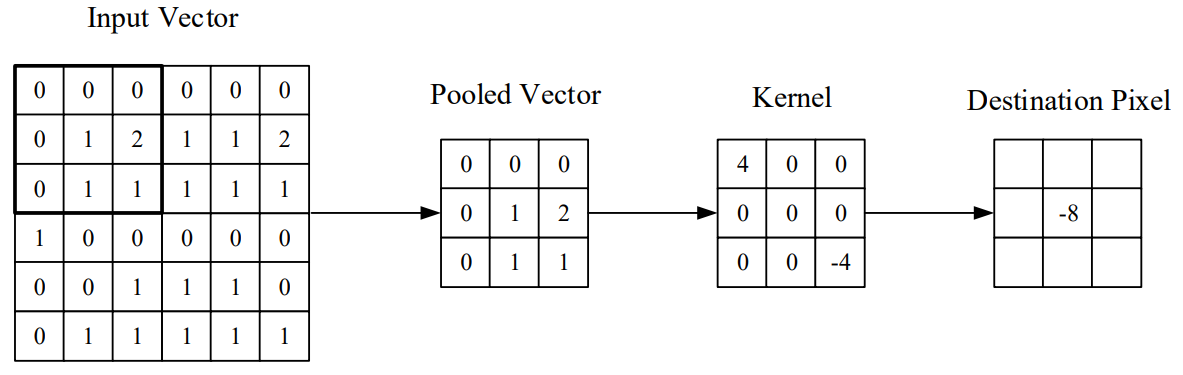
\includegraphics[width=0.8\textwidth]{images/KNNs/CNN Convolution.png}
      \caption{Beispiel für eine Faltung (engl.: Convolution) \cite{cnnsIntroduction}}
      \label{fig:convolution}
\end{figure}

Zunächst wird der Kernel beispielsweise auf die Teilmatrix \emph{links oben} der Eingangsmatrix angewendet. In Abbildung \ref{fig:convolution} ist dies visualisiert. Der betrachtete Teil der Eingangsmatrix wird hier als \emph{Pooled Vector} bezeichnet. Hierauf wird der Kernel, in diesem Fall ein sogenannter \emph{3x3-Kernel}, angewendet. Es wird also das Skalarprodukt der Werte mit dem gleichen Index aus dem \emph{Pooled Vector} und dem Kernel berechnet. In diesem Fall:
